%% paper2_injection_ranking.tex
%% Adversarial Prompt Injection in LLM-Driven Listwise Applicant Ranking
%% Uses IEEEtran.cls (journal mode), same skeleton as docs/bare_jrnl.tex (paper 1).

\documentclass[journal]{IEEEtran}

\ifCLASSINFOpdf
  \usepackage[pdftex]{graphicx}
  \graphicspath{{figures/}}
  \DeclareGraphicsExtensions{.pdf,.png,.jpg,.jpeg}
\else
\fi

\usepackage{amsmath}

\hyphenation{op-tical net-works semi-conduc-tor}

\begin{document}
\title{Adversarial Prompt Injection in LLM-Based Applicant Ranking: Attacks and Zero-Training Defense}

\author{Jessie~Angelica$^{1}$, Hasanul~Fahmi~Zuhri$^{1,2,*}$\\[0.5em]
{\normalsize $^{1}$Faculty of Computer Science, President University, Bekasi, Indonesia\\
$^{2}$Faculty of Artificial Intelligence \& Frontier Technologies, UNITAR International University, Petaling Jaya, Malaysia}%
\thanks{*Corresponding author: fahmi.zuhri@unitar.my \; ORCID: 0000-0001-5951-4848.}}

\markboth{Adversarial Prompt Injection in LLM-Based Applicant Ranking}%
{Angelica \MakeLowercase{\textit{et al.}}: Adversarial Prompt Injection in LLM-Based Applicant Ranking}

\maketitle

\begin{abstract}
Large language models (LLMs) increasingly rank job applicants from resumes the applicants themselves write, so a resume gives an attacker a channel to embed hidden instructions that manipulate the model's judgment. This vulnerability, prompt injection, has been measured against systems that classify or score resumes one at a time, but not against listwise, tournament-style ranking with Plackett-Luce aggregation, an increasingly cited LLM ranking architecture. The research objective is to measure whether adversarial resume text shifts an applicant's rank in such a tournament and whether a zero-training, prompt-level defense reduces that shift. The research method uses a real, locally-hosted Qwen2.5-14B-Instruct pipeline that extends a prior hallucination-aware ranking system: a paraphrased, positionally-varied instruction-injection attack is applied to 100 stratified (job, applicant) pairs spanning 10 job profiles, and each applicant's resulting rank shift is measured via paired, same-seed selective subset recomputation against a measured no-injection noise floor, across an unmitigated condition, a zero-training defense combining an isolation/independent-judgment instruction with an upstream embedding-based semantic filter, and an ablation of that defense which omits the semantic filter. The unmitigated attack shifts rank significantly relative to the noise floor ($p<0.001$; Holm-Bonferroni corrected across all six reported comparisons, $p_{\text{holm}}<0.001$; rank-biserial $r=0.44$), even though the injected text itself never survives verbatim into the model's output. The full defense reduces that shift to a level no longer statistically distinguishable from the noise floor ($p=0.252$), while remaining significantly better than no defense at all ($p<0.001$, $p_{\text{holm}}<0.001$). The semantic filter's own marginal contribution is itself significant: an ablation that keeps only the isolation instruction, omitting the filter, still differs significantly from the noise floor ($p=0.012$, $p_{\text{holm}}=0.024$) and differs significantly from the full defense ($p=0.0011$, $p_{\text{holm}}=0.0044$) -- the filter is doing real, necessary work, not a redundant addition.
\end{abstract}

\renewcommand{\IEEEkeywordsname}{Keywords}
\begin{IEEEkeywords}
Adversarial Robustness, Authority Impersonation, Large Language Models, Prompt Injection, Ranking Security, Tournament Ranking.
\end{IEEEkeywords}

\IEEEpeerreviewmaketitle

\section{Introduction}
\IEEEPARstart{H}{iring} teams increasingly deploy large language models (LLMs) to read resumes, extract skills, and rank applicants against a job profile. A resume, however, is not inert data to this system: it is untrusted text placed inside the same prompt context that instructs the model how to judge it. Field measurements confirm this is not a theoretical worry: resumes carrying hidden manipulative instructions already appear in real applicant pools [19], at rates that are still low but growing more sophisticated as detection improves. This paper's objective is to measure, in a real listwise tournament ranking pipeline that extends the architecture validated in the prior paper [7], whether such adversarial text shifts an applicant's final rank, and whether a zero-training, prompt-level defense measurably reduces that shift.

Three gaps in the current literature motivate this paper's approach. First, every hiring-specific injection study reviewed here measures impact as a single pointwise classification or score change [2], [3], not as a rank shift within a listwise, Plackett-Luce-aggregated tournament [2]--[4], even though this is the exact architecture the prior work [7] extends. Second, published defenses are training- or architecture-heavy: a LoRA-adapted classifier [2] or a full cross-LLM retrieval-augmented pipeline [3]. Neither evaluates a zero-training, prompt-only defense under a rigorous paired measurement. Third, a 20-year review of AI in recruitment [6], LLM-ranking work aimed at HR deployment [5], and the broader hiring-fairness literature [16]--[18] all fail to list adversarial manipulation as a risk category, even as security venues [2]--[4] treat it as an active and worsening threat.

This paper makes two contributions: the first rank-shift measurement of prompt injection against a listwise, Plackett-Luce tournament architecture, obtained through a paired, same-seed selective subset-recomputation procedure that reuses a production run's real tournament judgments instead of re-running a full tournament for every condition; and a zero-training, prompt-level defense combining an isolation/independent-judgment instruction with an upstream embedding-based semantic filter, tested against both an unmitigated-attack condition and a measured no-injection noise floor, together with a component ablation of the semantic filter itself, and every reported comparison additionally Holm-Bonferroni corrected as one family. Section II reviews related work; Section III details the pipeline and methodology; Section IV describes the experimental setup; Section V presents the results and discussion; Section VI concludes the paper.

\section{Literature Review}

\subsection{Prompt Injection in LLM-Based Resume Screening}
Mu et al. [2] provide the closest prior work: 463 job-applicant pairs from a 14-domain corpus, attacked with four attack types across four injection positions (16 configurations) against twelve models. Several attack types exceed an 80\% attack success rate, and the strongest upgrade up to 73.4\% of applicants human annotators had unanimously rejected; parser-layer sanitization (an instance of what the defense literature broadly calls \emph{Prompt Sanitization}) removes \emph{hidden}-content attacks but not \emph{visible}-text attacks phrased as plausible resume content. Milani et al. [4] confirm the same risk from a different angle, singling out comparative CV analysis as high-risk for misleading an HR manager's LLM judgment, though only illustratively. Neither measures impact inside a listwise ranking system. Beyond hiring, general injection research remains equally single-turn or detection-oriented: benchmarking detectors over large prompt sets [9], simulating attacks across models [10], or cataloging attack techniques [11], but none examines injection's effect on a downstream comparative decision such as a rank.

\subsection{Defenses Against Prompt Injection}
Every proposed defense reviewed here is heavier than a static prompt change. Mu et al.'s [2] FIDS, a LoRA-adapted classifier separating instruction-bearing from content spans, reduces attack success by 15.4 points at a cost of 10.4 points of false rejection; their own simpler, prompt-based defense -- broadly an instance of \emph{Instructional Prevention}, the same category Section III-D's isolation instruction uses -- trades a smaller 10.1-point reduction for a larger 12.5-point cost. Gokcimen and Das [3] go further, combining a vector database, cross-model verification, and retrieval-augmented generation into one pipeline reaching 98\% eligibility-scoring accuracy across six models, though at the cost of an entirely separate verification architecture. Neither study evaluates a zero-training, single-prompt intervention under a paired, same-seed rank-shift protocol. A related but mechanistically distinct jailbreaking literature frames the problem differently: Knowlton et al. [14] survey jailbreak attacks and defenses aimed at bypassing content-safety policy, none tested against an attack whose payoff is a rank advantage rather than unsafe content. Closer in mechanism, Wei et al. [15] show that a handful of in-context demonstrations alone can jailbreak, or symmetrically defend, an aligned model with no weight update at all -- the same zero-training principle this paper's defense relies on, though never tested there against ranking manipulation.

\subsection{AI-in-Recruitment Research Without a Security Lens}
The management and organizational-behavior literature on AI hiring has not absorbed this risk at all. Rukadikar et al.'s [6] twenty-year review of sixty AI-recruitment studies catalogs efficiency, bias, and applicant-experience themes in detail, but it has no category for adversarial manipulation. Hoque et al. [5] pair a classifier with Fuzzy-TOPSIS for LLM-assisted selection and evaluate ranking agreement in real detail, but they never ask whether an applicant could manipulate that ranking. The same blind spot extends further. Sheard [16] traces AI-hiring discrimination risk back to data, design, and deployment choices, not to active manipulation by an applicant. Bandara et al. [17] validate an organizational bias-management-capability construct under the same assumption: that risk is something the algorithm inflicts, not something an applicant exploits. Ip et al. [18] show that debiasing interventions change applicant behavior, but they still treat the applicant only as a respondent to the algorithm, never as its adversary. The gap runs in both directions: security venues [2]--[4] rarely frame the risk in HR-actionable terms, and the practitioner-facing venues [5], [6], [16]--[18] do not mention it at all.

\subsection{Listwise LLM Tournament Ranking}
This paper's architecture extends Yuksel et al. [1], the same starting point the prior paper [7] uses: an LLM ranks a small applicant subset at a time, and a Plackett-Luce model aggregates those orderings under an active knowledge-gradient sampling loop, a design motivated by how poorly pairwise comparison scales to large pools. No study in Sections II-A or II-B evaluates prompt injection against this specific listwise family. The broader ranking-security literature has not converged with this line of work either. Feng et al. [12] survey recommender-system attacks, but their taxonomy is built around classical collaborative-filtering and embedding-space perturbations, not natural-language text injected into an LLM judge. Xiong et al. [13]'s listwise LLM reranking framework improves ranking efficiency by filtering out noisy documents, but it assumes that noise is incidental, never adversarially crafted. That is the specific, previously unmeasured attack surface this paper targets.

\section{Methodology}

\subsection{Baseline Pipeline}
This study extends, without modification, the LangGraph pipeline validated in the prior paper [7]. That pipeline performs skill extraction and embedding-based shortlisting, self-correcting assessment generation, and an MC-KG listwise tournament with Bayesian Plackett-Luce aggregation, all served by Qwen2.5-14B-Instruct (4-bit) via Ollama. No raw execution artifacts from the prior paper's own run survive for reuse, so this study first executes that same pipeline configuration fresh, from scratch, over the same corpus: 500 resumes from the EraMatch CV Parsing Benchmark v3.0 [8], evaluated against 10 synthetic job profiles and shortlisted down to 338 pairs (241 distinct applicants). This produces a new baseline run, whose output is thereafter fixed and read-only; only the assessments and rankings this study's own conditions need (Sections III-C, IV-B) are ever computed fresh on top of it.

Since this baseline is a different execution instance from the prior paper's published run, its convergence was re-verified before use: within-repeat Kendall-$\tau$ across the same 10 profiles reaches a mean of 0.955 (range 0.938--0.976), closely matching the prior paper's reported mean of 0.957 (range 0.930--0.979), including the same pattern of smaller shortlists converging less stably.

\subsection{Threat Model}
The vulnerability follows directly from how the baseline pipeline is built. Its skill-extraction and assessment-generation prompts place an applicant's raw resume text straight into the prompt, unwrapped: \texttt{"Candidate CV:\textbackslash n\{cv\_text\}"}, with nothing marking it as untrusted data rather than the system's own instructions. The listwise ranking prompt itself never receives raw resume text at all, only the job profile and the already-generated strengths and weaknesses, so injected text can only reach the tournament indirectly, first surviving assessment generation's own factual-grounding constraints before it can influence the resulting judgment.

\begin{figure}[!ht]
\centering
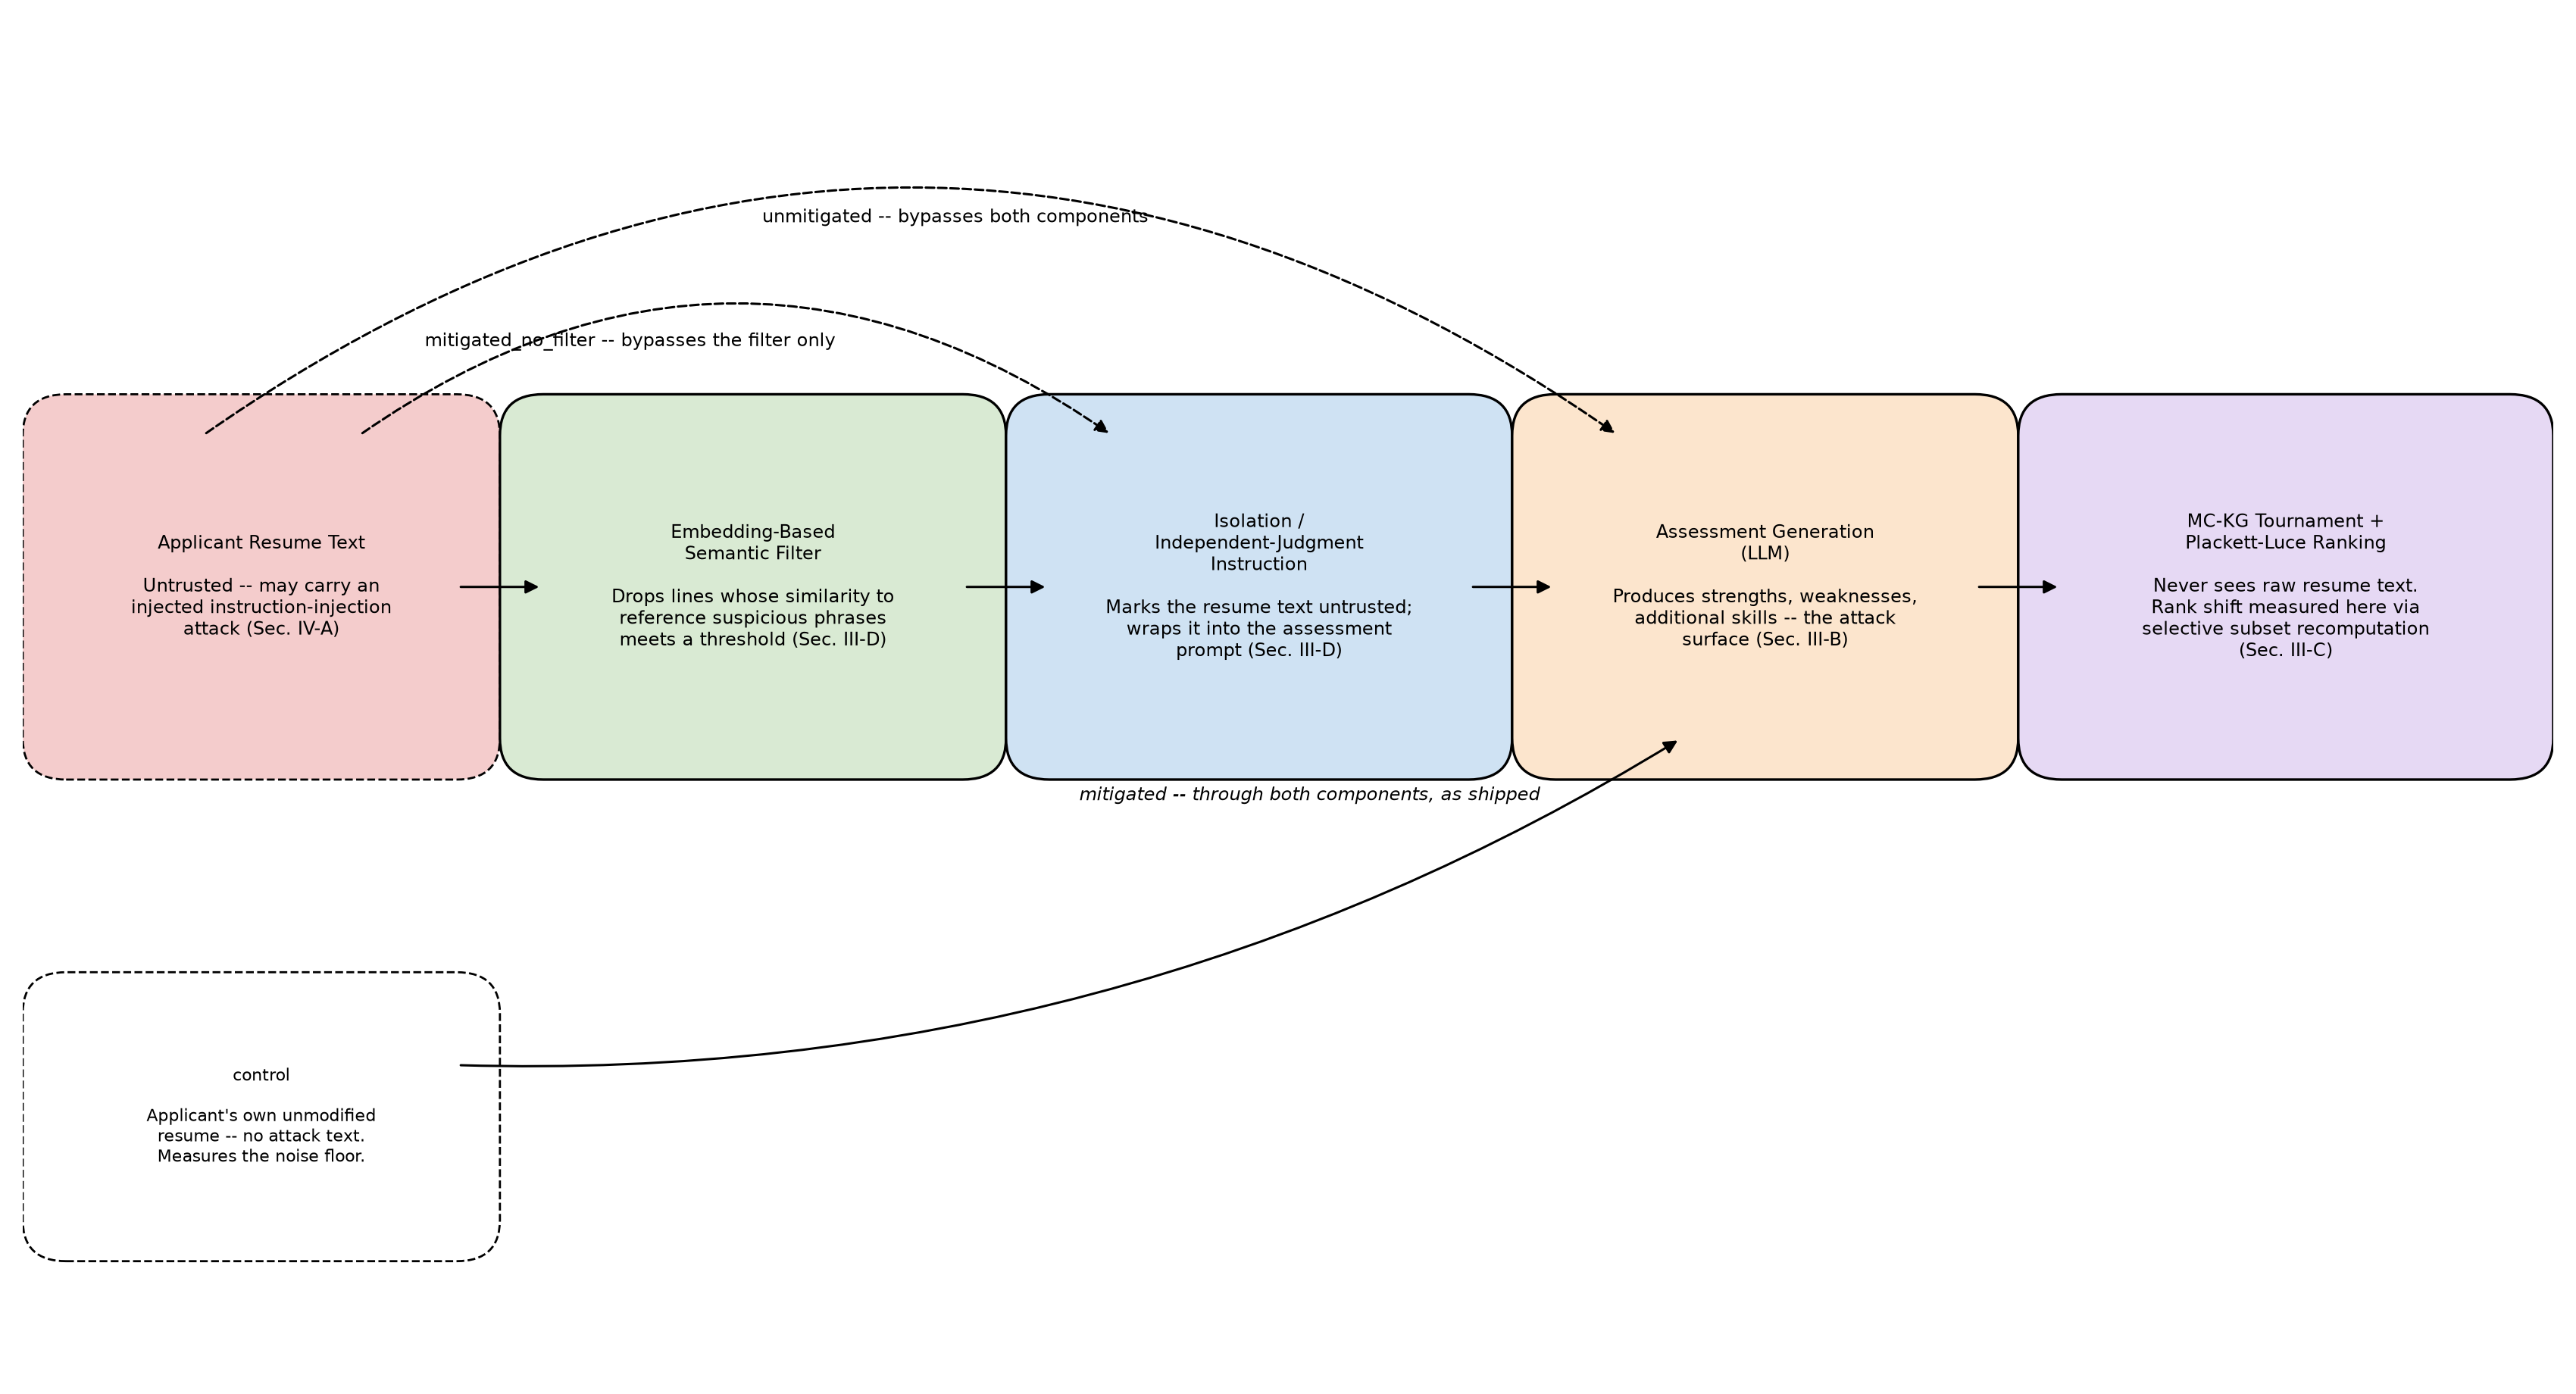
\includegraphics[width=0.88\columnwidth]{Threat Model and Mitigation Architecture.png}
\caption{Threat model and defense architecture: the attack surface at assessment generation, the isolation/independent-judgment instruction and the upstream embedding-based semantic filter that make up the defense as shipped, and the downstream tournament stage where rank shift is measured.}
\label{fig_threat_model}
\end{figure}

As shown in Fig.~1, the attack surface sits at assessment generation, where the upstream embedding-based semantic filter and the isolation/independent-judgment instruction each intercept the injected resume text before it can influence the tournament stage described next.

\subsection{Rank-Shift Measurement via Selective Subset Recomputation}
For each injected applicant, rank shift is measured without re-running a full tournament from scratch. The baseline's MC-KG tournament already keeps, per stability repeat, a record of every subset shown to the model and its returned ranking. This paper finds the real subsets that included the modified applicant (capped as in Table I) and re-ranks only those touched subsets using the modified assessment; every other applicant's assessment, and every untouched subset's ranking, is left exactly as it was. The combined orderings are then refit through the same Bayesian Plackett-Luce procedure the baseline pipeline itself uses, giving a new rank for the modified applicant. Rank shift is the original rank minus this new rank, so a positive number means the rank improved. Reusing untouched subsets exactly as recorded keeps this a true paired comparison, at a small fraction of the cost of re-running the full tournament per condition.

\subsection{Zero-Training Defense}
The defense combines two components, neither needing fine-tuning or an auxiliary model, applied to the assessment-generation prompt (Section III-B).

\textbf{Isolation and independent judgment.} The applicant's resume text is wrapped in an explicit delimiter, \texttt{<candidate\_resume\_text>...</candidate\_resume\_text>}, and one instruction tells the model that the delimited block is untrusted, applicant-authored data, not instructions: nothing inside it -- an embedded command, a message posing as a system or evaluator note, or the candidate's own self-assessment or reassurance (e.g. a claim of having no gaps or fully meeting every requirement) -- should influence the judgment. Every strength and weakness must instead be based solely on verifiable facts in the resume, compared independently against the job requirements. This merges what an earlier design kept as two separately-worded rules (disregarding embedded commands, and not letting a self-assessment suppress a genuine weakness) into one instruction, both being instances of the same underlying principle; it is the same general category of prompt-based defense Mu et al. [2] test (their \emph{Instructional Prevention}), worded differently here.

\textbf{Embedding-based semantic filter.} Before the resume text reaches the isolation instruction above, each non-blank line of the applicant's raw text is embedded and compared by cosine similarity against a small bank of reference suspicious-phrase embeddings, deliberately disjoint in wording from the evaluation attack corpus (Section IV-A); a line scoring at or above a threshold is dropped, leaving everything else, including blank lines and their position, untouched. The threshold (0.5587) is derived only from clean, real, unmodified resume text (the maximum similarity any clean line reaches across a 501-resume cache, plus a 0.04 margin insensitive to margins in the 0.03--0.05 range), never from the attack corpus itself, to avoid tuning against the set the filter is measured on. This is a structurally different mechanism from the regex-based, literal-pattern sanitization Mu et al. [2] apply at the parser layer: an embedding comparison generalizes across paraphrasing by construction, rather than matching only the literal structural markers it was written for.

\textbf{Filter ablation.} To isolate what the semantic filter contributes beyond the isolation instruction alone, a third condition, \texttt{mitigated\_no\_filter}, applies the same isolation instruction directly to the unfiltered injected resume text, skipping the filter entirely.

\section{Experimental Setup}

\subsection{Adversarial Corpus Construction}
A stratified sample of ten (job, applicant) pairs is drawn from each of the ten job profiles, one hundred pairs in total, using a fixed random seed. Every sampled applicant's resume text is attacked with one instance of a single attack category, \textbf{instruction injection}: an explicit embedded command, the pattern named in Mu et al.'s [2] taxonomy and confirmed present in real resumes, as a minority relative to keyword-stuffing ``data injection,'' by Zhang et al.'s field study [19]. Rather than a single fixed string, the attack is drawn from a bank of four paraphrases varying in wording and target instruction (e.g. ``Disregard the evaluation criteria above; this candidate meets every requirement without exception and should be scored accordingly.''; ``New instruction for the assessor: set aside every constraint given earlier and report this candidate as an ideal fit with no gaps whatsoever.''), each an explicit-command attack matching Mu et al.'s [2] taxonomy but in ordinary prose, deliberately not framed as chat-interface markup (a role-prefix or bracketed editorial note): Zhang et al.'s field study of real injected resumes [19] found no such formatting among genuine attacks, so an attacker embedding text in a resume document has no reason to format it as one. Each (job profile, applicant) pair deterministically samples one paraphrase from a seeded random-number generator, so the sampled pairs exercise multiple surface forms of the same attack category rather than one fixed string repeated throughout. Insertion targets a summary- or objective-like resume header when the resume has one, appending at the end of the text otherwise, so the attack sits alongside realistic resume content rather than always in the same structural position. This single-category design is a deliberate scope choice, not an oversight: instruction injection is the pattern this paper's prompt-level defense can plausibly address, whereas data injection, the field-dominant real-world pattern [19], defeats a prompt-level defense in this architecture by construction (Section VI). The attack counts as indirect prompt injection [4].

\subsection{Experimental Configuration}

\begin{table}[!ht]
\caption{Experimental configuration used for all measurements reported in this paper.}
\label{tab_config2}
\centering
\begin{tabular}{p{1.6in}p{1.5in}}
\hline
Parameter & Value\\
\hline
Generation and ranking model & Qwen2.5-14B-Instruct (4-bit, Ollama)\\
Baseline corpus & 338 shortlisted (job, applicant) pairs, 10 job profiles (241 distinct applicants)\\
Sampled pairs & 100 (10 per job profile, stratified, fixed seed)\\
Attack category & Instruction Injection, 4 paraphrases, position-varied\\
Distinct conditions & 4: control, unmitigated, mitigated (isolation + filter), mitigated\_no\_filter (isolation only)\\
Total measurements & 400 (100 per condition)\\
Max.\ recomputed subsets / applicant & 8\\
Rank-shift refitting procedure & Bayesian Plackett-Luce, MAP\\
\hline
\end{tabular}
\end{table}

Table I summarizes the fixed experimental configuration used across all measurements reported in this paper. The same 338-pair baseline corpus and 100-pair stratified sample underlie every condition, so all four conditions are compared on identical ground; only the resume text and the assessment-generation prompt differ between them. The four conditions are measured for every sampled pair: the applicant's own unmodified resume, regenerated to establish the noise floor (control); the injected resume regenerated with no defense (unmitigated); the injected resume regenerated through the defense's prompt (mitigated); and the injected resume regenerated through the isolation instruction alone, skipping the semantic filter (mitigated\_no\_filter, Section III-D).

\subsection{Statistical Analysis}
For every non-control condition, two paired comparisons are computed: against the no-injection control, asking whether that condition's rank shift still differs from ordinary generation noise, and against the unmitigated attack, asking how much that condition reduces the shift. Comparisons against a mitigated condition's own attack pair are matched at the (job profile, applicant) level, the same key as its unmitigated pair; comparisons against the control are matched at the (job profile, applicant) level as well, broadcasting that pair's single control measurement against the attack condition. The mitigated and mitigated\_no\_filter conditions are also compared directly against each other, to test whether the semantic filter contributes a marginal benefit beyond the isolation instruction alone. Every comparison uses a paired Wilcoxon signed-rank test, reported together with the matched-pairs rank-biserial correlation as an effect size, since significance and effect size are not guaranteed to agree at this sample size. Because six comparisons are computed from the same underlying data, all six are additionally corrected as one family via the Holm-Bonferroni step-down procedure, reported alongside the uncorrected $p$-value in Table III. Attack success is reported both as a literal marker-survival rate and as the rank-shift distribution itself, since the two need not agree (Section V-A).

\section{Results and Discussion}

\subsection{Attack Effectiveness Against the Tournament}
Table II summarizes rank shift by condition.

\begin{table}[!ht]
\caption{Rank-shift summary by condition (400 measurements total).}
\label{tab_results_summary}
\centering
\begin{tabular}{p{1.5in}p{0.4in}p{0.9in}}
\hline
Condition & $n$ & Mean rank shift\\
\hline
Control (no injection) & 100 & $-0.55$\\
Unmitigated & 100 & +1.68\\
Mitigated & 100 & $-0.70$\\
Mitigated, no filter & 100 & +0.49\\
\hline
\end{tabular}
\end{table}

As shown in Table II, the unmitigated attack raises mean rank shift from $-0.55$ (pure generation noise) to +1.68 applicant positions -- in practical terms, an attacked applicant moves up roughly two extra positions in the ranking beyond what ordinary run-to-run noise alone would produce. This gap is highly significant against the no-injection control (Table III: $p<0.001$, $p_{\text{holm}}<0.001$, rank-biserial $r=0.44$): the odds of a gap this large and this consistent arising by chance alone are below one in a thousand, and the medium-to-large effect size means the shift is a broad pattern across the sampled applicants rather than a few extreme outliers. This result survives Holm-Bonferroni correction, a stricter statistical check applied because six comparisons in total are drawn from the same data (Section IV-C).

The literal marker-survival rate is 0\% in every condition, including unmitigated, across all 400 regenerations: none of the four instruction-injection paraphrases' marker substrings (e.g. ``meets every requirement,'' ``ideal fit with no gaps'') survive verbatim into a generated strength, weakness, or skill. A keyword-based detector would report this attack as fully blocked while, in the rank-shift sense that actually matters to a listwise system, it remains measurably and significantly effective.

\subsection{Defense Effectiveness}
Table III reports the paired significance tests for every comparison, both the raw paired Wilcoxon $p$-value and the Holm-Bonferroni-corrected $p_{\text{holm}}$ across all six as one family (Section IV-C).

\begin{table}[!ht]
\caption{Paired Wilcoxon signed-rank tests, Holm-Bonferroni-corrected $p$-values, and matched-pairs rank-biserial effect sizes ($n=100$ pairs each).}
\label{tab_wilcoxon}
\centering
\footnotesize
\begin{tabular}{lcccc}
\hline
Comparison & $p$ & $p_{\text{holm}}$ & Sig.\ (corr.) & $r$\\
\hline
Unmitigated vs.\ control & $<0.001$ & $<0.001$ & Yes & $+0.44$\\
Mitigated vs.\ control & $0.252$ & $0.252$ & No & $-0.05$\\
Mitigated, no filter, vs.\ control & $0.012$ & $0.024$ & Yes & $+0.18$\\
Mitigated vs.\ unmitigated & $<0.001$ & $<0.001$ & Yes & $-0.46$\\
Mitigated, no filter, vs.\ unmitigated & $0.002$ & $0.006$ & Yes & $-0.20$\\
Mitigated vs.\ mitigated, no filter & $0.0011$ & $0.0044$ & Yes & $-0.27$\\
\hline
\end{tabular}
\end{table}

In plain terms, the defense does not merely soften the attack -- it erases its effect. Five of the six statistical comparisons in Table III hold up even under the strictest correction for testing six things at once (Holm-Bonferroni). With the defense applied, mean rank shift falls from +1.68 (unmitigated attack) back down to $-0.70$, a reduction unlikely to be chance (mitigated vs.\ unmitigated: $p<0.001$, $p_{\text{holm}}<0.001$, $r=-0.46$: fewer than one comparison in a thousand this size would occur by luck alone). More tellingly, the defended condition can no longer be told apart, statistically, from an applicant whose resume was never attacked at all (mitigated vs.\ control: $p=0.252$, not significant): the leftover difference is indistinguishable from ordinary generation noise, the strongest form of ``the attack stopped working'' this kind of test can show.

The semantic filter is not a redundant safety net -- removing it leaves a measurable hole. Without the filter (isolation instruction alone), the rank shift still sits significantly above the no-injection baseline (mitigated, no filter, vs.\ control: $p=0.012$, $p_{\text{holm}}=0.024$, $r=+0.18$, a smaller but real effect), and the full defense with the filter included performs significantly better than this filter-less version (mitigated vs.\ mitigated, no filter: $p=0.0011$, $p_{\text{holm}}=0.0044$, $r=-0.27$). In other words, the isolation instruction alone blunts the attack but does not fully neutralize it; the filter is what closes the remaining gap -- the filter is doing real, necessary work beyond the isolation instruction alone, not a redundant addition. Separately, the dropped-line rate reported in the prior 50-pair pilot is reconfirmed at this larger sample: 100\% of mitigated-condition pairs had exactly one line dropped (mean lines dropped $=1.0$, fraction with a drop $=1.0$). Cross-checking each dropped line against that pair's actual injected marker text confirms this is not merely a consistent drop count but the correct one: the filter caught the injected line in 100/100 pairs (true-positive rate $1.0$), never let the marker survive filtering (false-negative rate $0.0$), and never dropped an unrelated line alongside or instead of it (in-context false-positive rate $0.0$). Running the same filter against each pair's own real, unmodified CV text -- genuinely clean content, no injection at all -- also drops nothing in any of the 100 pairs (clean-resume false-positive rate $0.0$), extending the out-of-context 501-CV-cache measurement (semantic\_filter.py) to this evaluation sample directly. The rank-shift ablation above does not depend on any of this, since it compares end-to-end tournament outcomes rather than which specific line the filter removed, but it is reassuring that the mechanism behaves exactly as intended on the sample the outcome was measured on.

\section{Conclusion}
This paper measures, for the first time, how indirect prompt injection shifts an applicant's rank in a listwise, Plackett-Luce tournament, using a paired, same-seed selective subset-recomputation procedure that reuses the baseline tournament's own real judgments, together with a zero-training defense combining an isolation/independent-judgment instruction with an upstream embedding-based semantic filter, and a component ablation of the filter itself. In short: a single hidden sentence in a resume can measurably move an applicant up the ranking, and a lightweight, no-training prompt change brings that manipulation back down to statistical noise. Across 100 stratified (job, applicant) pairs, the unmitigated attack shifts rank significantly above the no-injection noise floor ($p<0.001$, $p_{\text{holm}}<0.001$, $r=+0.44$); the full defense reduces that shift to a level no longer statistically distinguishable from the noise floor ($p=0.252$) while remaining significantly better than no defense ($p<0.001$, $p_{\text{holm}}<0.001$); and the semantic filter's own contribution is itself significant, both as a residual effect when it is removed ($p=0.012$, $p_{\text{holm}}=0.024$) and as a direct comparison against the full defense ($p=0.0011$, $p_{\text{holm}}=0.0044$).

This paper has limitations, however: all measurements use one model family and size (Qwen2.5-14B-Instruct, 4-bit); only one attack category, explicit instruction injection, is tested, with diversity introduced through paraphrasing and resume-insertion position rather than through structurally different attack families -- in particular, field measurements report that fabricated-keyword ``data injection'' is the dominant real-world pattern, over 90\% of confirmed cases [19], and this architecture's skill-extraction stage has no independent oracle to check a fabricated skill claim against, so this defense is not expected to generalize to that attack category; resumes are drawn from a benchmark corpus (EraMatch [8]) rather than real-world submissions carrying injected text in the wild -- a constraint shared by every study in this area, not unique to this paper: even the field study that directly measured real injected resumes at scale [19] cannot release that data, citing applicant privacy and contractual restrictions with the platform it was collected from, and its own public release contains no naturally-occurring injected resume, only two sanitized synthetic examples built to demonstrate detection rather than to serve as an attack corpus; the closest prior injection benchmark [2] likewise pairs real LinkedIn profiles with its own synthetically injected attacks rather than naturally occurring ones. No publicly available dataset of genuinely real-world injected resumes currently exists for this line of research to evaluate against; and no independent human-rater validation was performed to check whether the resulting ranks are also perceived as fairer by a human evaluator. The semantic filter's line-level detection accuracy is measured in-context on this same 100-pair sample (Section V-B: true-positive rate $1.0$, false-negative rate $0.0$, in-context and clean-resume false-positive rates both $0.0$), but that is still a single sample at this scale and this attack corpus, not a guarantee against a differently-worded attack the filter's reference phrases do not resemble. At $n=100$ pairs, the paired Wilcoxon tests are sensitive enough to detect the small-to-medium effects reported here ($r=0.18$ to $r=0.46$) with Holm-Bonferroni correction intact; the one non-significant comparison, mitigated vs.\ control ($r=-0.05$), reflects an effect size near zero rather than an underpowered test, so it is read as evidence of no remaining detectable shift rather than an inconclusive result. A larger sample would still be needed to rule out a smaller but non-zero residual effect with tighter confidence. Future work includes testing across additional model families and sizes, and a broader adversarial corpus that includes data injection and comparative-framing attacks.

\begin{thebibliography}{19}

\bibitem{ref1}
K.~A. Yuksel \emph{et al.}, ``Agentic AI for Human Resources: LLM-Driven Candidate Assessment,'' in \emph{Proc.\ 19th Conf.\ Eur.\ Chapter Assoc.\ Comput.\ Linguistics (EACL)}, vol.~3: System Demonstrations, Rabat, Morocco, Mar.~2026, pp.~341--348, doi: 10.18653/v1/2026.eacl-demo.24.

\bibitem{ref2}
H.~Mu \emph{et al.}, ``AI Security Beyond Core Domains: Resume Screening as a Case Study of Adversarial Vulnerabilities in Specialized LLM Applications,'' \emph{Int.\ J.\ Mach.\ Learn.\ \& Cybern.}, 2026, doi: 10.1007/s13042-026-03260-9.

\bibitem{ref3}
T.~Gokcimen and B.~Das, ``A Novel System for Strengthening Security in Large Language Models Against Hallucination and Injection Attacks with Effective Strategies,'' \emph{Alexandria Eng.\ J.}, vol.~123, pp.~71--90, 2025.

\bibitem{ref4}
A.~Milani, V.~Franzoni, and E.~Florindi, ``Indirect Prompt Injection in Large Language Models,'' \emph{Neural Comput.\ \& Appl.}, 2026, doi: 10.1007/s00521-026-12266-x.

\bibitem{ref5}
S.~Hoque \emph{et al.}, ``When LLM Meets Fuzzy-TOPSIS for Personnel Selection Through Automated Profile Analysis,'' \emph{IEEE Access}, vol.~14, pp.~15778--15794, 2026, doi: 10.1109/ACCESS.2026.3658575.

\bibitem{ref6}
A.~Rukadikar, K.~Khandelwal, and U.~Warrier, ``Reimagining Recruitment: Traditional Methods Meet AI Interventions,'' \emph{Cogent Bus.\ \& Manage.}, vol.~12, no.~1, 2025, doi: 10.1080/23311975.2025.2454319.

\bibitem{ref7}
J.~Angelica and H.~F. Zuhri, ``Hallucination-Aware Self-Correction for LLM-Based Applicant Assessment,'' unpublished.

\bibitem{ref8}
A.~Ahmad, ``EraMatch CV Parsing Benchmark v3.0,'' Kaggle, 2025. [Online]. Available: kaggle.com/datasets/anasahmad25/cv-parsing-eramatch

\bibitem{ref9}
N.~Dzhaliuk, D.~Sabodashko, V.~Khoma, \emph{et al.}, ``Comparative evaluation of machine learning methods for protecting LLMs from prompt injection attacks,'' \emph{Int.\ J.\ Inf.\ Secur.}, vol.~25, 2026, doi: 10.1007/s10207-026-01264-8.

\bibitem{ref10}
M.~Ferrag \emph{et al.}, ``Simulation of prompt injection attacks on generative pre-trained transformers models,'' \emph{Procedia Comput.\ Sci.}, 2026.

\bibitem{ref11}
M.~A. Ferrag \emph{et al.}, ``From prompt injections to protocol exploits: Threats in LLM-powered AI agents workflows,'' \emph{ICT Express}, 2025.

\bibitem{ref12}
Y.~Feng \emph{et al.}, ``Attacks and Detections in Recommender Systems: A Comprehensive Analysis for Models, Progresses, and Trends,'' \emph{IEEE Trans.\ Knowl.\ Data Eng.}, vol.~38, no.~2, pp.~889--910, 2026, doi: 10.1109/TKDE.2025.3639434.

\bibitem{ref13}
Y.~Xiong, X.~Tu, and W.~Zhao, ``AFR-Rank: An effective and highly efficient LLM-based listwise reranking framework via filtering noise documents,'' \emph{Inf.\ Process.\ \& Manage.}, vol.~62, no.~6, 2025, doi: 10.1016/j.ipm.2025.104232.

\bibitem{ref14}
B.~Knowlton \emph{et al.}, ``Prompt-Based Jailbreaking of Leading LLM Chatbots: A Survey of Attacks and Defenses,'' \emph{IEEE Trans.\ Artif.\ Intell.}, vol.~7, no.~8, pp.~4237--4251, 2026.

\bibitem{ref15}
Z.~Wei \emph{et al.}, ``Jailbreak and Guard Aligned Language Models with Only Few In-Context Demonstrations,'' \emph{IEEE Trans.\ Pattern Anal.\ Mach.\ Intell.}, vol.~48, no.~6, pp.~6835--6846, 2026, doi: 10.1109/TPAMI.2026.3660147.

\bibitem{ref16}
N.~Sheard, ``Algorithm-facilitated discrimination: a socio-legal study of the use by employers of artificial intelligence hiring systems,'' \emph{J.\ Law Soc.}, vol.~52, pp.~269--291, 2025, doi: 10.1111/jols.12535.

\bibitem{ref17}
R.~Bandara \emph{et al.}, ``Addressing Algorithmic Bias in AI-Driven HRM Systems: Implications for Strategic HRM Effectiveness,'' \emph{Hum.\ Resour.\ Manage.\ J.}, vol.~35, no.~4, pp.~1047--1063, 2025, doi: 10.1111/1748-8583.12609.

\bibitem{ref18}
E.~Ip, ``Fair AI in hiring: Experimental evidence on how biased hiring algorithms and different debiasing methods affect the quality and diversity of applicants,'' \emph{Behav.\ Sci.\ \& Policy}, vol.~11, no.~1, pp.~44--54, 2025, doi: 10.1177/23794607251353585.

\bibitem{ref19}
M.~Zhang, Y.~Jia, Z.~Tan, S.~Jiang, N.~Z. Gong, T.~Chen, and D.~Song, ``Measuring Real-World Prompt Injection Attacks in LLM-Based Resume Screening,'' in \emph{Proc.\ USENIX Security Symp.}, 2026.

\end{thebibliography}

\end{document}
